Distributed systems typically consist of two or more components that communicate \emph{asynchronously} by sending and receiving messages through a network layer~\cite{lamport1978time}. When a component receives a message, it responds by executing a predefined \emph{message handler}. This handler consists of a sequence of program statements that might update the internal state of the component, send a message to another component in the system, or even create an entirely new component.

As an example of a distributed system, Figure~\ref{fig:azurestore} shows the top-level components of Azure Storage vNext, a distributed extent management system for Windows Azure that is used in production inside Microsoft. Azure Storage vNext consists of multiple extent managers, extent nodes and a remote procedure call (RPC) communication engine. Each extent manager is responsible for managing a subset of the extent nodes. Each extent node is responsible for storing its corresponding extent in a local storage. Finally, the RPC engine is responsible for sending messages across the network, and enqueuing any received messages in the inbox queue of the corresponding node. This system is described in more details in Section~\ref{sec:cases:azurestore}.

\subsection{Bugs in distributed systems}
\label{sec:overview:bugs}

In a distributed system, message handlers can interleave in arbitrary order, because of the asynchronous nature of message-based communication. To complicate matters further, unexpected failures are the norm in production: nodes in a cluster might fail at any moment, and thus programmers have to implement sophisticated mechanisms that can deal with these failures and recover the state of the system. Moreover, with multicore machines having become a commodity, individual components of a distributed system are commonly implemented using multithreaded code, which adds another source of nondeterminism.

\begin{figure}[t]
\centering
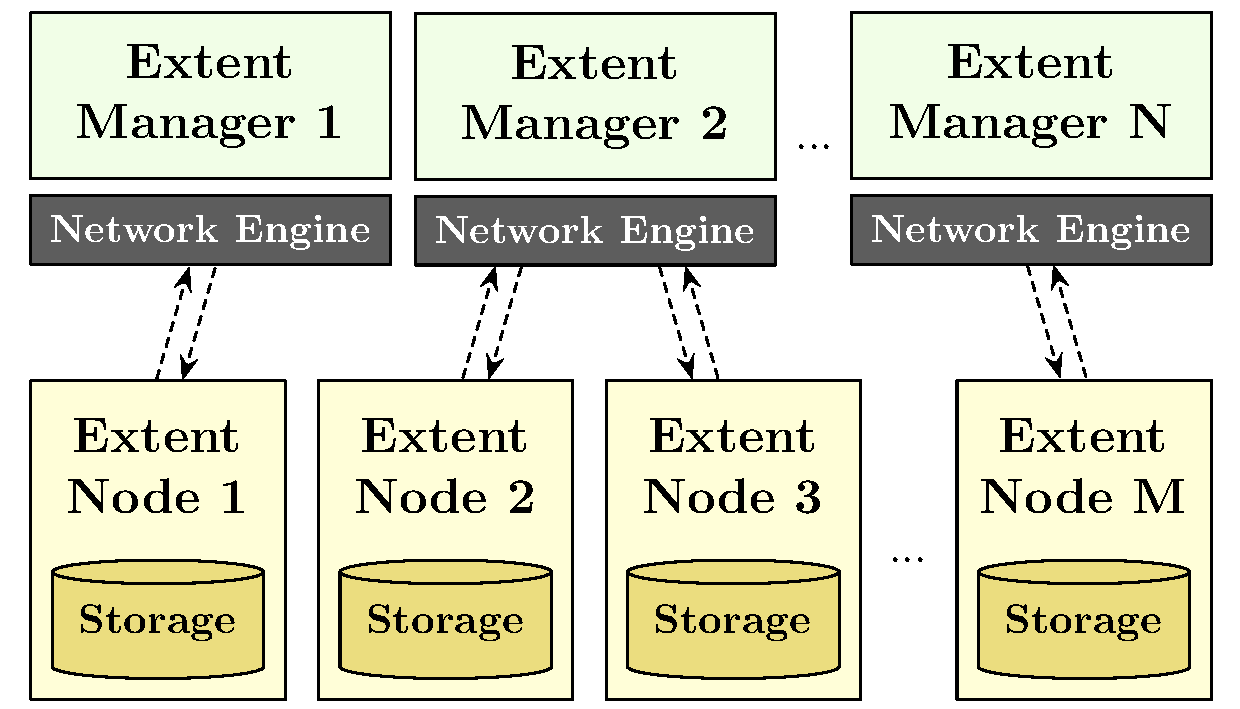
\includegraphics[width=\linewidth]{img/azurestore}
\caption{Top-level components of a distributed extent management system for Windows Azure.}
\label{fig:azurestore}
\end{figure}

All these sources of nondeterminism (as well as nondeterminism due to timeouts, message losses and client requests) can easily create \emph{heisenbugs}~\cite{gray1986computers, musuvathi2008finding}, which are corner-case bugs that are difficult to detect, diagnose and fix, without using advanced \emph{asynchrony-aware} testing techniques.
%
The ideal testing tool should be able to work on unmodified systems, capture and control all possible sources of nondeterminism, systematically inject faults in the right places, and explore all feasible execution paths. However, this is easier said than done when testing production systems.

There are two types of bugs that developers of distributed systems are mostly interested in finding: \emph{safety} and \emph{liveness} property violations~\cite{lamport1977proving}.


\begin{description}
\item[Safety] A safety property checks that an erroneous program state is \emph{never} reached, and is satisfied if it \emph{always} holds in each possible program execution.

\item[Liveness] A liveness property checks that some progress \emph{will} happen, and is satisfied if it \emph{always eventually} holds in each possible program execution.
\end{description}

\noindent
A safety property can be specified using an \emph{assertion} that fails if the property gets violated in some program state. As an example, in Azure Storage vNext we assert that whenever a message gets dequeued there must be an action that can handle the received message. Note that this safety property is not specific to Azure Storage vNext, and can be used in any system based on message passing.

Liveness properties are much harder to specify and check since they apply over entire program executions and not just individual program states. The liveness property that is being checked in the Azure Storage vNext system is that a user-defined $N$ number of extent nodes must be always eventually available with the latest extent. 

Normally, liveness checking requires the identification of an infinite fair execution that never satisfies the liveness property~\cite{schuppan2004efficient, musuvathi2008fair}. Prior work~\cite{schuppan2004efficient} has proposed that assuming a program with finite state space, a liveness property can be converted into a safety property. Other researchers proposed the use of heuristics and only exploring finite executions of an infinite state space system using random walks to identify if a liveness property is violated~\cite{killian2007life}.

\PDComment{Quickly say how we found Cheng's bug?}

\subsection{Testing distributed systems today}
\label{sec:overview:testing}

Although a significant amount of research has been conducting during the past few decades on how to test distributed systems,

only a small amount of this research was successful enough to be picked up by industry.

\PDComment{How cheng was testing his code before and how after -- high level, pretty picture}

\subsection{The \psharp approach}
\label{sec:overview:psharp}

\PDComment{Insert fancy \psharp picture}

The \psharp~\cite{deligiannis2015psharp} project provides an \emph{event-driven asynchronous programming} language and a \emph{concurrency unit testing} framework for developing highly-reliable distributed systems.

The \psharp language is an extension of \csharp that enables asynchronous programming using communicating state-machines. \psharp machines can interact asynchronously by sending and receiving events, an approach commonly used to develop distributed systems. This programming model is similar to actor-based approaches provided by other asynchronous programming languages (e.g. Scala~\cite{odersky2008programming} and Erlang~\cite{armstrong1996erlang}).

A \psharp machine consists of an input queue for received events, states, state transitions, event handlers, fields and methods. Machines run concurrently with each other, each executing an event handling loop that dequeues an event from the input queue and handles it by invoking an appropriate event handler. This handler might update a field, create a new machine, or send an event to another machine. In \psharp, a send operation is non-blocking; the message is simply enqueued into the input queue of the target machine, and it is up to the operating system scheduler to decide when to dequeue an event and handle it.

Because \psharp is built on top of \csharp, the programmer can blend \psharp and \csharp code; this not only lowers the overhead of learning a new language, but also allows \psharp to easily integrate with legacy code. Another advantage is that the programmer can use the familiar programming and debugging environment of Visual Studio.

The second core component of the \psharp project is a concurrency unit testing framework that is embedded in the \psharp runtime. This framework allows the event schedulings of a \psharp program to be explored in a controlled manner, facilitating deterministic replay of bugs.

\psharp is available as open-source\footnote{\url{https://github.com/p-org/PSharp}} and is currently used by various teams in Microsoft to develop and test distributed protocols and systems.

%The \psharp language belongs to the same family of languages as P~\cite{desai2013p}.

\PDComment{mention dependency injection pattern?}